\chapter{Common objects}

\section{Date class}

Developer: Simon Leger

\subsection{Approach}

In order to work with financial data, where one of the most important factors is time, we 
needed a serious object to handle it.  This is why we came up with the idea of writing our own date class 
even if it was not really required in the project. This date class has been designed especially for financial use 
since one can find features common in finance such as business day and day count conventions.

In this approach the dates are stored as long integers where 1 is the first of January 1900.  Dates can also be easily created or accessed by giving the day, month and year. There is a whole set of powerful functions to get the last day of the month or to count the number of days 
between two dates according to a certain convention.

\subsection{Implementation}

There is a base class called Date and then a derived class called UsDate.  UsDate is able to use any function of the base 
class.  Additionally there is a boolean function which returns whether a specific day is a US business day or not. 
This could be adapted for any country by adding other sub classes.


\section{Interpolator}

Developer: Joseph Perez

\subsection{Approach}
We implemented a 1D and 2D quadratic interpolator.

The interpolator required for the implied volatility surface returns the degree two polynomial for each
maturity which best fits the computed implied volatilities.  However we can make two observations
\begin{enumerate}
	\item the shape of the surface of the S$\&$P now is a skewed surface more than a smile
	\item we want our interpolator to return a function that matches the known implied volatilities
\end{enumerate}
These requirements are not satisfied with the method described above.  Accordingly, we decided to implement another one. As the shape is rather smooth we do local interpolation: at a given point we evaluate the degree two polynomial which goes through the nearest known points. 


\subsection{Implementation}
We adapted the general implementation of polynomial interpolation from Numerical Recipes to focus only on polynomials of degree two.
In 1D, only one polynomial of degree two goes through three points. Our algorithm returns the evaluation of this polynomial on a fourth point without computing its coefficients.
In 2D, we use the same methodology. First we run three interpolations on one axis and then a last one on the other axis.

Outside our boundaries we force the interpolator to return the value of the nearest point.  This means that the interpolated curve or surface is flat outside the frontiers.

\section{Matrix}

Developer: Yann Renoux

\subsection{Approach}

Though we have decided to manage our data with valarrays to avoid dealing with pointers, the use of a matrix class was justified by two important applications in the yield curve and rainbow option sections of the project.

\subsubsection{The yield curve}

As part of the requirements for constructing the yield curve, we had to transform the swap rates into zero coupon rates in order to have an homogeneous set of points and be able to back out all the needed methods that a yield curve should have (most importantly spot rate to maturity, discount factors, forward rates). As shown in the yield curve section, changing from swap rates to zero coupon rates requires inverting a lower triangular matrix. Since coding the Gauss method for valarrays did not really make sense, a matrix class, based on Tony Veit's class was added to the project. Indeed, for such a basic tool, there is no need to re-invent the wheel. This class provides all the necessary methods and more to handle matrices generally.  Specifically, it made it easier to invert the swap rates matrix to get the zero coupons.

\subsubsection{Dealing with correlations - Cholesky decomposition}

On the section on rainbow options, we have to deal with correlated Brownian motions (see this section for more details). Though the formula is straightforward for a set of two underlyings, we aimed at making our classes as reusable as possible which motivated us to support more than two underlying assets.  The main issue was to sample $n$ independent normal distributions and recorrelate them all at the same time to produce correlated asset prices. One method to accomplish this is Cholesky decomposition of the correlation matrix. This method transforms a square matrix into a product of a lower triangular matrix multiplied by its transpose based on the eigenvalues decomposition without having to solve for them. Therefore, we added the Cholesky algorithm to the existing matrix class to be able to use it in the rainbow options class.


\subsection{Implementation}

There is nothing magic in this matrix class, it just has a double** as a private member to store the data, and then provides all the usual operators (redefined) for linear algebra, such as multiplication by a scalar or a matrix, transposition, inversion, etc. Additionally, the sum of columns, rows, diagonal matrix are available, as well as a "$<<$" operator to output the matrix. This was really useful in verifying the Cholesky decomposition results against what we expected.


\section{Cummulative bivariate normal distribution}

Developer: Yann Renoux

\subsection{Approach}

The rainbow options closed formulas need to use the Cummulative bivariate normal distribution function. The same way we ahve used the polynomial approximation, we have computed the polynomial approximation for $\mathcal{BN}(a,b,\r)$. We have used the approach discribed in Hull's \textit{Options, Futures and Other Derivatives - 5th Edition}, pages 245-246.

\subsection{Results and effects of the correlation}

The correlation mainly impacts the inflexion point steepness around $(a,b)=(0,0)$ as the polynomial approximation is a Taylor expansion. The more the correlation the steeper the inflexion point. The results are as follows:

\begin{figure}
\begin{center}    
        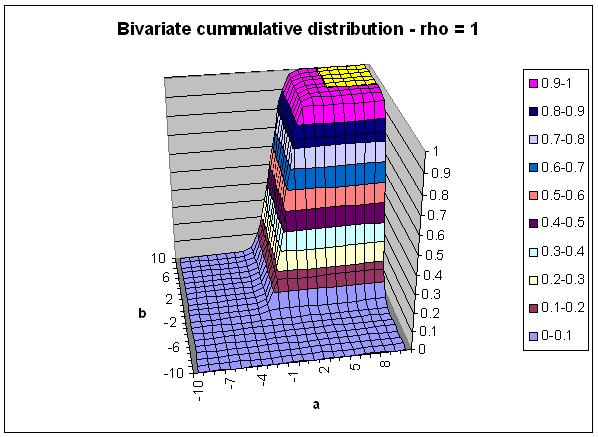
\includegraphics[width=10cm]{Bivn1.jpg}
        \caption{Cumulative bivariate normal distribution for $\r=1$}
\end{center}
\end{figure}

\begin{figure}
\begin{center}    
        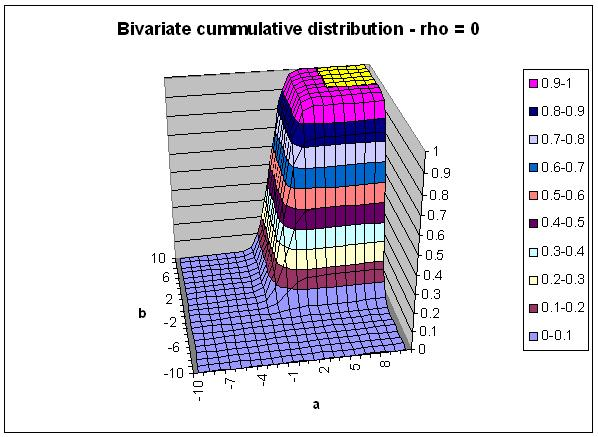
\includegraphics[width=10cm]{Bivn0.jpg}
        \caption{Cumulative bivariate normal distribution for $\r=0$}
\end{center}
\end{figure}

\begin{figure}
\begin{center}    
        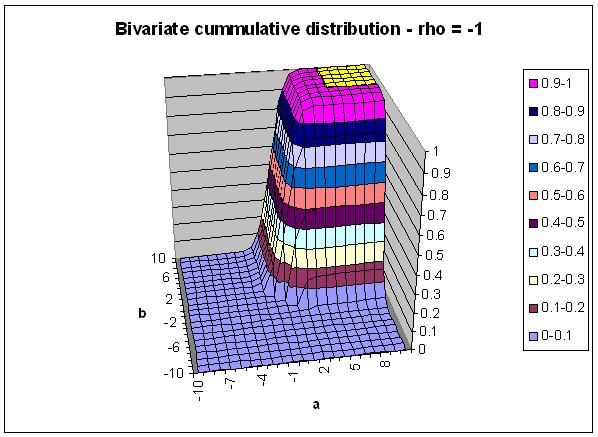
\includegraphics[width=10cm]{BivnNeg1.jpg}
        \caption{Cumulative bivariate normal distribution for $\r=-1$}
\end{center}
\end{figure}


\newpage

\section{FileReader}

Developer: Aloke Mukherjee

\subsection{Approach}

The FileReader class simplifies the task of working with structured data.  Some examples of structured data used in the project include swap and zero rates, option prices and credit spreads.  We wanted to be able to store this data in a simple comma-delimited text format so that it could be easily changed in a text editor.  The FileReader bridges the gap between this human-readable format and the data structures used in the project.  

\subsection{Implementation}

The FileReader relies on the CSVParser class developed by Mayukh Bose to read comma-delimited files.  Reusing this class allowed us to avoid some of the headaches involved with parsing text.  The CSVParser class has a simple but powerful interface that pipes in data from the file and pipes it out as an appropriate data type.  Some customization was required to allow the CSVParser to understand terreneuve-specific types like dates, credit spread types.  Once the data has been transformed from text into valid data types, FileReader can construct the internal data structures which are required to instantiate classes such as credit curves or a volatility surface.  

The other useful function of FileReader is discovering and caching the location of the common data directory.  The test routines use the cached value to locate their test data files.